\section{Definirea problemei}
% enuntul intrebarii
În această secțiune vom prezenta problma fiecărui puzzle.
\newline


\subsection{Domino - Seven Squares}

\begin{enumerate}
    \item Prima Problemă\newline\newline
 Așezarea a șapte cadre pătrate cu toate cele 28 de piese de domino. Dominourile cu același număr de puncte se întâlnesc.\newline
    \item A doua Problemă\newline\newline
Așezarea a șapte cadre pătrate cu toate cele 28 de piese de domino, astfel încât sumele numerelor de puncte să fie aceleași pe toate cele patru laturi. \newline
Suma este 4 + 4 + 2 = 2 + 2 + 6 = 6 + 1 + 3 = 3 + 3 + 4 = 10.\newline
\end{enumerate}

\begin{figure}[h]
    \centering
    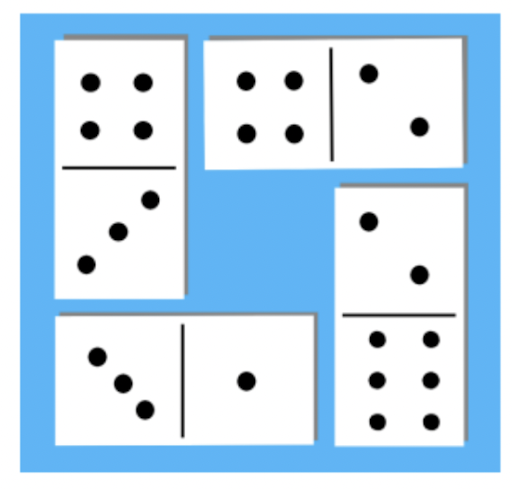
\includegraphics[width=8cm]{text/images/pic3.png}\\
    \caption{Seven Squares}
\end{figure} \newline
După cum se observă și în poză, fiecare 2 capete vecine 3-3 , 4-4 și 2-2, au același număr. Dar, 6!=1.
Se poate găsi o posibilitate pentru a îndeplini toate condițiile?
Vom afla la implementare.

\pagebreak
\subsection{The Resistance - Spy View}

\begin{enumerate}
    \item Prima Problemă\newline\newline
Din punctul de vedere al echipei de spioni, cea mai mare problemă din jocul este încercarea de a afla cine sunt ceilalți spioni. Pentru a avea succes, echipa de spionaj trebuie să lucreze împreună și să-și coordoneze eforturile fără a se lăsa în fața echipei Rezistența.\newline
    \item A doua Problemă\newline\newline
O altă problemă pentru echipa de spionaj este să încerce să saboteze misiunile echipei de Rezistență fără a fi prins. Echipa de spionaj își poate folosi voturile pentru a încerca să blocheze propunerile de misiune, dar dacă sunt prea evidente, echipa Rezistenței poate deveni suspicioasă și poate începe să-și dea seama cine sunt spionii. Aceasta înseamnă că echipa de spionaj trebuie să fie atentă și strategică în modul în care își folosesc voturile și să încerce să saboteze misiunile. \newline

\end{enumerate}

\begin{figure}[h]
    \centering
    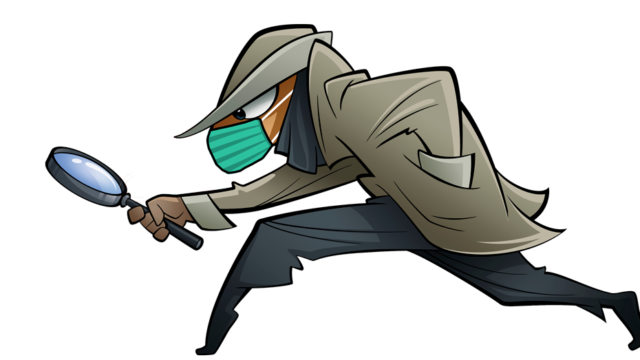
\includegraphics[width=8cm]{text/images/pic4.png}\\
\end{figure} \newline\newline

\newline\newlineÎn general, echipa de spionaj se confruntă cu o serie de provocări în jocul Rezistenței, inclusiv încercarea de a-și da seama cine sunt colegii lor spioni, lucrul împreună fără a se dezvălui și sabotarea eforturilor echipei Rezistență fără a fi prins. Aceste provocări pot face jocul captivant și plin de suspans și necesită ca echipa de spionaj să-și folosească inteligența și gândirea strategică pentru a reuși.

\pagebreak